\documentclass{beamer}
\usepackage{ctex, hyperref}
\usepackage{caption}
\usepackage[T1]{fontenc}

\usepackage[ruled,linesnumbered]{algorithm2e}

% other packages
\usepackage{latexsym,amsmath,xcolor,multicol,booktabs,calligra}
\usepackage{graphicx,pstricks,listings,stackengine}

\author[Sean Chao]{學~~~~~~生:Sean~Chao\vskip 5pt 指導老師:XXX~教授}
\title{NTHU Beamer Theme}
\subtitle{碩士學位論文模板}
\institute{清華大學資訊系統與應用研究所}
\date{\today}
\usepackage{Tsinghua}

% defs
\def\cmd#1{\texttt{\color{red}\footnotesize $\backslash$#1}}
\def\env#1{\texttt{\color{blue}\footnotesize #1}}
\definecolor{deepblue}{rgb}{0,0,0.5}
\definecolor{deepred}{rgb}{0.6,0,0}
\definecolor{deepgreen}{rgb}{0,0.5,0}
\definecolor{halfgray}{gray}{0.55}

\lstset{
    basicstyle=\ttfamily\small,
    keywordstyle=\bfseries\color{deepblue},
    emphstyle=\ttfamily\color{deepred},    % Custom highlighting style
    stringstyle=\color{deepgreen},
    numbers=left,
    numberstyle=\small\color{halfgray},
    rulesepcolor=\color{red!20!green!20!blue!20},
    frame=shadowbox,
}


\begin{document}
% 圖/Fig.
\captionsetup[figure]{labelfont={bf},name={Fig.},labelsep=period}
% 標題頁
\begin{frame}
    \titlepage
    \begin{figure}[htpb]
        \begin{center}
            
\includegraphics[width=0.15\linewidth]{pic/nthu-1.eps}
        \end{center}
    \end{figure}
\end{frame}

% Outline
\begin{frame}{Outline}
    \tableofcontents[sectionstyle=show,subsectionstyle=show/shaded/hide,subsubsectionstyle=show/shaded/hide]
\end{frame}

\section{介紹}

\subsection{簡介}

\begin{frame}{Why \LaTeX}
    \begin{itemize}
        \item \LaTeX 廣泛用於學術界,期刊會議論文
    \end{itemize}
    \begin{table}[h]
        \centering
        \begin{tabular}{c|c}
            Microsoft\textsuperscript{\textregistered}  Word & \LaTeX \\
            \hline
            文字處理工具 & 專業排版軟件 \\
            高級功能不易掌握 & 進階難,但一般用不到 \\
            處理長文檔需要豐富經驗 & 和短文檔處理相同 \\
            花費大量時間調格式 & 無需擔心格式 \\
            公式排版差 & 擅長公式排版 \\
            二進制,兼容性差 & 文本文件,穩定 \\
            付費 & 免費 \\
        \end{tabular}
    \end{table}
\end{frame}

\begin{frame}{Beamer}
    \begin{itemize}
        \item Beamer是一個用於建立演示文稿 \LaTeX 的文件類
        \item 預設生成PDF檔案用於演示,其動態效果依靠建立多頁幻燈片實現
    \end{itemize}
\end{frame}

\subsection{美化主題}

\begin{frame}{主題來源}
    \begin{itemize}
        \item 調整配色
        \item 一些 \LaTeX{} 原本的
        \item 一些 \href{http://far.tooold.cn/post/latex/beamertsinghua}{\color{deepred}{原始Tsinghua}} \cite{1}的,已經失效
        \item 主要基於 \href{https://www.overleaf.com/latex/templates/thu-beamer-theme/vwnqmzndvwyb}{\color{deepred}{修改版Tsinghua}} \cite{2}修改
        \item 參考 \href{https://github.com/SunYanCN/Latex-Beamer-Template}{\color{deepred}{中文Beamer模板}} \cite{3}新增功能
    \end{itemize}
\end{frame}

\begin{frame}{其他}
    \begin{itemize}
        \item 原始模板功能可以參考
        \url{https://www.latexstudio.net/archives/4051.html}
        \item Beamer的用法,節選自\href{https://stu.cs.tsinghua.edu.cn/~harry/latex-talk.pdf}{\color{deepred}{如何使用LATEX排版论文}}\cite{4}
    \end{itemize}
\end{frame}

\section{教學}
\subsection{舉例}
\subsubsection{數學公式}
\begin{frame}{公式}
    \begin{exampleblock}{無編號公式} % 加 * 
        加 * 號
        \begin{equation*}
            J(\theta) = \mathbb{E}_{\pi_\theta}[G_t] = \sum_{s\in\mathcal{S}} d^\pi (s)V^\pi(s)=\sum_{s\in\mathcal{S}} d^\pi(s)\sum_{a\in\mathcal{A}}\pi_\theta(a|s)Q^\pi(s,a)
        \end{equation*}
    \end{exampleblock}
\end{frame}

\begin{frame}{公式}
    \begin{exampleblock}{多行多列公式\footnote{如果公式中有文字出現,請用$\backslash$mathrm\{\} 或者$\backslash$text\{\} 包含,不然就會變成$clip$,在公式中看起來比$\mathrm{clip}$ 難看非常多}}
        用 \textbackslash \textbackslash 分隔,若不編號則加上\textbackslash nonumber
        % 使用 & 分隔
        \begin{align}
            y & =d & z & =1 \\
            y_{12} & =bx^{2}+cx+d & z & =x^{2}+x+1\nonumber \\
            y(x) & =ax^{3}+bx^{2}+cx+d & z & =x^{3}+x^{2}+x+1 \\
            Q_\mathrm{target}&=r+\gamma Q^\pi(s^\prime, \pi_\theta(s^\prime)+\epsilon) \\
            \epsilon&\sim\mathrm{clip}(\mathcal{N}(0, \sigma), -c, c)\nonumber
        \end{align}
    \end{exampleblock}
\end{frame}

\begin{frame}{公式}
    \begin{exampleblock}{編號多行公式}
        % Taken from Mathmode.tex
        \begin{multline}
            A=\lim_{n\rightarrow\infty}\Delta x\left(a^{2}+\left(a^{2}+2a\Delta x+\left(\Delta x\right)^{2}\right)\right.\label{eq:reset}\\
            +\left(a^{2}+2\cdot2a\Delta x+2^{2}\left(\Delta x\right)^{2}\right)\\
            +\left(a^{2}+2\cdot3a\Delta x+3^{2}\left(\Delta x\right)^{2}\right)\\
            +\ldots\\
            \left.+\left(a^{2}+2\cdot(n-1)a\Delta x+(n-1)^{2}\left(\Delta x\right)^{2}\right)\right)\\
            =\frac{1}{3}\left(b^{3}-a^{3}\right)
        \end{multline}
    \end{exampleblock}
\end{frame}
\subsubsection{圖}
\begin{frame}{圖片排版}
    % From thuthesis user guide.
    \begin{minipage}[c]{0.3\linewidth}
        \psset{unit=0.8cm}
        \begin{pspicture}(-1.75,-3)(3.25,4)
            \psline[linewidth=0.25pt](0,0)(0,4)
            \rput[tl]{0}(0.2,2){$\vec e_z$}
            \rput[tr]{0}(-0.9,1.4){$\vec e$}
            \rput[tl]{0}(2.8,-1.1){$\vec C_{ptm{ext}}$}
            \rput[br]{0}(-0.3,2.1){$\theta$}
            \rput{25}(0,0){%
            \psframe[fillstyle=solid,fillcolor=lightgray,linewidth=.8pt](-0.1,-3.2)(0.1,0)}
            \rput{25}(0,0){%
            \psellipse[fillstyle=solid,fillcolor=yellow,linewidth=3pt](0,0)(1.5,0.5)}
            \rput{25}(0,0){%
            \psframe[fillstyle=solid,fillcolor=lightgray,linewidth=.8pt](-0.1,0)(0.1,3.2)}
            \rput{25}(0,0){\psline[linecolor=red,linewidth=1.5pt]{->}(0,0)(0.,2)}
%           \psRotation{0}(0,3.5){$\dot\phi$}
%           \psRotation{25}(-1.2,2.6){$\dot\psi$}
            \psline[linecolor=red,linewidth=1.25pt]{->}(0,0)(0,2)
            \psline[linecolor=red,linewidth=1.25pt]{->}(0,0)(3,-1)
            \psline[linecolor=red,linewidth=1.25pt]{->}(0,0)(2.85,-0.95)
            \psarc{->}{2.1}{90}{112.5}
            \rput[bl](.1,.01){C}
        \end{pspicture}
    \end{minipage}\hspace{1cm}
    \begin{minipage}{0.5\linewidth}
        \medskip
        %\hspace{2cm}
        \begin{figure}[h]
            \centering
            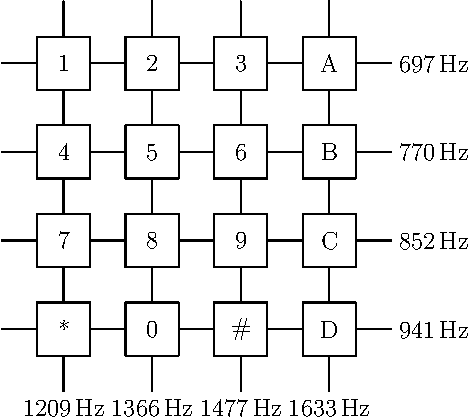
\includegraphics[height=.4\textheight]{pic/dtmf.pdf}
        \end{figure}
    \end{minipage}
\end{frame}

\begin{frame}{文字排版}
  \begin{columns}
    \begin{column}{.45\textwidth}
      \begin{figure}[h]
        \centering
        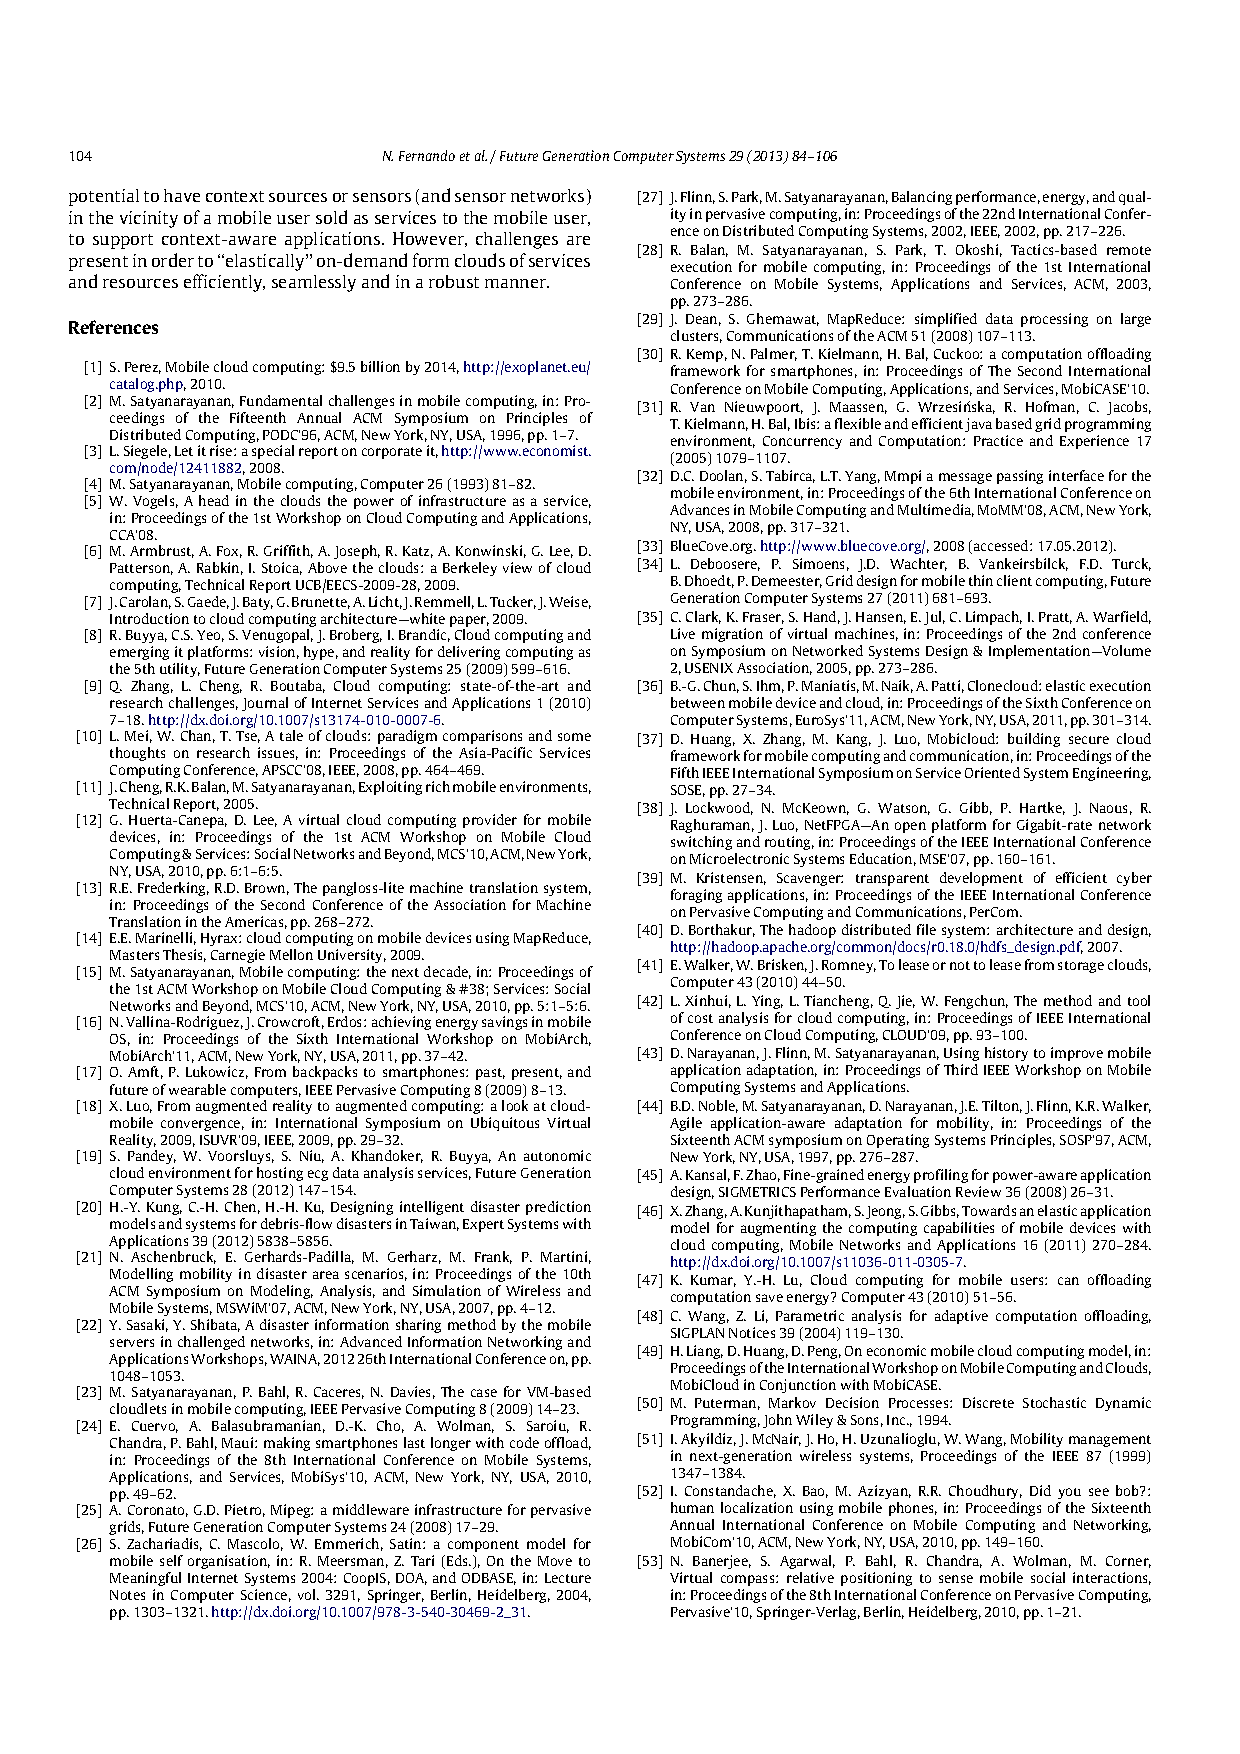
\includegraphics[width=.8\textwidth]{pic/references.pdf}
      \end{figure}
    \end{column}
    \begin{column}{.45\textwidth}
      \begin{figure}[h]
        \centering
        
\includegraphics[width=.8\textwidth]{pic/shapepar.pdf}
      \end{figure}
    \end{column}
  \end{columns}
\end{frame}

\subsection{常用指令}
\begin{frame}[fragile]{結構}
  \lstset{language=[LaTeX]TeX}
  \begin{lstlisting}[basicstyle=\ttfamily]
    \documentclass[a4paper]{article}
    % 文檔類型,如 article
    % []是選項,如 a4paper
    
    % 導言區
    \usepackage{graphicx} % 引用包
    \graphicspath{{fig/}} % 設定圖片位置

    \begin{document}
    正文
    \end{document}
  \end{lstlisting}
\end{frame}
\begin{frame}[fragile]{\LaTeX{}指令}
    \framesubtitle{\emph{Macro}、\emph{控制序列} (control sequence)}
    \begin{itemize}
        \item 簡單指令
          \begin{itemize}
            \item \verb|\指令|\\
                \verb|\songti 人民的意志| ~$\Rightarrow$ {\songti 人民的意志}
            \item \verb|\指令[可選參數]{必選參數}|\\
                \verb|\section[精簡標題]{這個題目實在太長了}|
          \end{itemize}
        \item 環境
          \begin{columns}[c]
            \begin{column}{0.45\textwidth}
    \begin{lstlisting}[basicstyle=\ttfamily]
\begin{equation*}
  a^2-b^2=(a+b)(a-b)
\end{equation*}
    \end{lstlisting}
            \end{column}\hspace{0.75em}
            \begin{column}{0.45\textwidth}
                $ a^2-b^2=(a+b)(a-b)$
            \end{column}
        \end{columns}
    \end{itemize}
\end{frame}
\begin{frame}[fragile]{\LaTeX{}常用指令}
    \begin{exampleblock}{簡單指令}
        \centering
        \footnotesize
        \begin{tabular}{llll}
            \cmd{chapter} & \cmd{section} & \cmd{subsection} & \cmd{paragraph} \\
            章 & 節 & 小節 & 帶題頭段落 \\\hline
            \cmd{centering} & \cmd{emph} & \cmd{verb} & \cmd{url} \\
            居中對齊 & 强调 & 原樣輸出 & 超連結 \\\hline
            \cmd{footnote} & \cmd{item} & \cmd{caption} & \cmd{includegraphics} \\
            注釋 & 列表條目 & 標題 & 插入圖片 \\\hline
            \cmd{label} & \cmd{cite} & \cmd{ref} \\
            標號 & 引用參考文獻 & 引用圖表、公式等\\\hline
        \end{tabular}
    \end{exampleblock}
    \begin{exampleblock}{環境}
        \centering
        \footnotesize
        \begin{tabular}{lll}
            \env{table} & \env{figure} & \env{equation}\\
            表格 & 圖片 & 公式 \\\hline
            \env{itemize} & \env{enumerate} & \env{description}\\
            無編號列表 & 有編號列表 & 描述 \\\hline
        \end{tabular}
    \end{exampleblock}
\end{frame}
\begin{frame}[fragile]{\LaTeX{} 無序列表舉例}
    \begin{minipage}{0.5\linewidth}
\begin{lstlisting}[language=TeX]
\begin{itemize}
  \item A \item B
  \item C
  \begin{itemize}
    \item C-1
  \end{itemize}
\end{itemize}
\end{lstlisting}
    \end{minipage}\hspace{1cm}
    \begin{minipage}{0.2\linewidth}
        \begin{itemize}
            \item A
            \item B
            \item C
            \begin{itemize}
                \item C-1
            \end{itemize}
        \end{itemize}
    \end{minipage}
    \medskip
\end{frame}
\begin{frame}[fragile]{\LaTeX{} 有序列表舉例}
    \begin{minipage}{0.5\linewidth}
\begin{lstlisting}[language=TeX]
\begin{enumerate}
  \item 巨佬 \item 大佬
  \item 萌新
  \begin{itemize}
    \item 瑟瑟發抖
  \end{itemize}
\end{enumerate}
\end{lstlisting}
    \end{minipage}\hspace{1cm}
    \begin{minipage}{0.3\linewidth}
        \begin{enumerate}
            \item 巨佬
            \item 大佬
            \item 萌新
            \begin{itemize}
                \item 瑟瑟發抖
            \end{itemize}
        \end{enumerate}
    \end{minipage}
\end{frame}
\begin{frame}[fragile]{\LaTeX{} 數學公式}
    \begin{columns}
        \begin{column}{.55\textwidth}
\begin{lstlisting}[language=TeX]
$V = \frac{4}{3}\pi r^3$

\[
  V = \frac{4}{3}\pi r^3
\]

\begin{equation}
  \label{eq:vsphere}
  V = \frac{4}{3}\pi r^3
\end{equation}
\end{lstlisting}
        \end{column}
        \begin{column}{.4\textwidth}
            $V = \frac{4}{3}\pi r^3$
            \[
                V = \frac{4}{3}\pi r^3
            \]
            \begin{equation}
                \label{eq:vsphere}
                V = \frac{4}{3}\pi r^3
            \end{equation}
        \end{column}
    \end{columns}
    \begin{itemize}
        \item 詳細可查 \href{https://zh.wikipedia.org/wiki/Help:数学公式}{\color{deepred}{維基}}
        \item unicode-math包
    \end{itemize}
\end{frame}
\begin{frame}[fragile]{層次}
    \begin{columns}
        \begin{column}{.6\textwidth}
\begin{lstlisting}[basicstyle=\ttfamily\small]
\tableofcontents
\part{監督式學習}
\chapter{SVM}
\section{SVM簡介}
\subsection{SVM的歷史}
\subsubsection{SVM的誕生}
\paragraph{一些趣聞}
\subparagraph{第一個趣聞}
\end{lstlisting}
\end{column}
\begin{column}{.4\textwidth}
第一部分\quad 監督式學習\\
第一章\quad SVM \\
1. SVM簡介 \\
1.1 SVM的歷史 \\
1.1.1 SVM的誕生 \\
一些趣聞 \\
第一個趣聞
        \end{column}
    \end{columns}
\end{frame}
\begin{frame}[fragile]{列表}
    \begin{columns}
        \begin{column}{.6\textwidth}
\begin{lstlisting}[basicstyle=\ttfamily\small]
\begin{enumerate}
\item \LaTeX{}好處
  \begin{description}
    \item[好用] 體驗好
    \item[好看] 福音
  \end{description}
\item 還有呢?
  \begin{itemize}
    \item 好處 1
    \item 好處 2
  \end{itemize}
\end{enumerate}
\end{lstlisting}
        \end{column}
        \begin{column}{.4\textwidth}
{\small
\begin{enumerate}
\item \LaTeX{}好處
  \begin{description}
    \item[好用] 體驗好
    \item[好看] 爽
  \end{description}
\item 還有呢?
  \begin{itemize}
    \item 好處 1
    \item 好處 2
  \end{itemize}
\end{enumerate}
}
        \end{column}
    \end{columns}
\end{frame}
\begin{frame}[fragile]{交叉引用}
    \begin{itemize}
        \item 命名:圖片、表格、公式等\\
        \textbackslash label\{name\}
        \item 引用\\
        \textbackslash ref\{name\}
    \end{itemize}
\end{frame}
\begin{frame}[fragile]{交叉引用}
    \begin{columns}
        \column{.6\textwidth}
\begin{lstlisting}[language=TeX]
\begin{table}[htbp]
  \caption{編號與含義}
  \label{tab:number}
  \centering
  \begin{tabular}{cl}
    \toprule
    編號 & 含義 \\
    \midrule
    1 & 4.0 \\
    2 & 3.7 \\
    \bottomrule
  \end{tabular}
\end{table}
公式~(\ref{eq:vsphere})的編號
與含義請參見表~\ref{tab:number}。
\end{lstlisting}
        \column{.4\textwidth}
        \begin{table}[htpb]
            \centering
            \caption{編號與含義}
            \label{tab:number}
            \begin{tabular}{cl}\toprule
                編號 & 含義 \\\midrule
                1 & 4.0\\
                2 & 3.7\\\bottomrule
            \end{tabular}
        \end{table}
        \normalsize 公式~(\ref{eq:vsphere})的編號與含義請參見表~\ref{tab:number}。
    \end{columns}
\end{frame}
\begin{frame}{插入圖片}
    \begin{itemize}
        \item 向量圖 eps, ps, pdf
        \begin{itemize}
            \item Matlab / Excel 等另存pdf
            \item 不(完全)支援: .svg, .bmp
        \end{itemize}
        \item 點陣圖 png, jpg, tiff $\ldots$
        \begin{itemize}
            \item 應盡量避免
        \end{itemize}
    \end{itemize}
    \begin{figure}[htpb]
        \centering
        
\includegraphics[width=0.2\linewidth]{pic/nthu-16.eps}
        \caption{這個校徽就是向量圖(eps)}
    \end{figure}
\end{frame}

\begin{frame}{表格}
  \begin{itemize}
    \item 推薦使用工具轉出code:\href{https://www.tablesgenerator.com/latex_tables}{{\LaTeX{} Table Generator}}
  \end{itemize}
\end{frame}

\begin{frame}{演算法}
\begin{algorithm}[H]
	\caption{HOSVD}
	\small 
	\KwIn{HOSVD($\mathcal{X},R_{1},R_{2}.....R_{N}$) }
	\KwOut{ $\mathcal{G},A_{(1)},A_{(2)}......A_{(N)} $ }
	
	\For{$k=1$ to $N$ }
	{
		$A_{(n)}\leftarrow R_{n}$left singular matrix of $X_{(n)}$
	}
	$\mathcal{G}=\leftarrow \mathcal{X} \times A_{(1)}^{T} \times A_{(2)}^{T}...... \times A_{(N)}^{T}$\\
	\Return $\mathcal{G},A_{(1)},A_{(2)}......A_{(N)} $
\end{algorithm}
\end{frame}

\begin{frame}[fragile]{code}
HOSVD用Python實現:
\lstinputlisting[lastline=11,
language=Python,
frame=single,
caption=First 10 lines of Python code,
label=python]
{HOSVD.py}
\end{frame}

\begin{frame}[fragile]
  \frametitle{推薦包}
  \setlength{\leftmarginii}{1.5em}
  \vspace{-1.5em}
  \begin{multicols}{3}
    \begin{itemize}
      \item 必備
        \begin{itemize}
          \item \pkg{amsmath}
          \item \pkg{graphicx}
          \item \pkg{hyperref}
        \end{itemize}

      \item 樣式
        \begin{itemize}
          \item \pkg{caption}
          \item \pkg{enumitem}
          \item \pkg{fancyhdr}
          \item \pkg{footmisc}
          \item \pkg{geometry}
          \item \pkg{titlesec}
        \end{itemize}

      \item 數學
        \begin{itemize}
          \item \pkg{bm}
          \item \pkg{mathtools}
          \item \pkg{physics}
          \item \pkg{unicode-math}
        \end{itemize}

      \item 表格
        \begin{itemize}
          \item \pkg{array}
          \item \pkg{booktabs}
          \item \pkg{longtable}
          \item \pkg{tabularx}
        \end{itemize}

      \item 圖
        \begin{itemize}
          \item \pkg{float}
          \item \pkg{pdfpages}
          \item \pkg{standalone}
          \item \pkg{subfig}
          \item \pkg{pgf}/\pkg{tikz}
          \item \pkg{pgfplots}
        \end{itemize}

      \item 字體
        \begin{itemize}
          \item \pkg{newpx}
          \item \pkg{pifont}
          \item \pkg{fontspec}
        \end{itemize}

      \item 各種功能
        \begin{itemize}
          \item \pkg{algorithm2e}
          \item \pkg{beamer}
          \item \pkg{biblatex}
          \item \pkg{listings}
          \item \pkg{mhchem}
          \item \pkg{microtype}
          \item \pkg{minted}
          \item \pkg{natbib}
          \item \pkg{siunitx}
          \item \pkg{xcolor}
        \end{itemize}

      \item 多語言
        \begin{itemize}
          \item \pkg{babel}
          \item \pkg{polyglossia}
          \item \pkg{ctex}
          \item \pkg{xeCJK}
        \end{itemize}
    \end{itemize}
  \end{multicols}
  \vspace*{-0.5cm}
\end{frame}

\section{參考文獻}
\begin{frame}[allowframebreaks]
    \begin{block}{Note}
      如果參考文獻太多,可以使用tiny/scriptsize/footnotesize/small
      % \tiny\bibliographystyle{alpha}
    \end{block}
    \scriptsize\bibliographystyle{plain}
    \bibliography{ref}
\end{frame}

\section{End}
\begin{frame}{Q\&A}
    \begin{center}
    	\LARGE \centering  Questions?  %問
    \end{center}
\end{frame}
\begin{frame}
    \begin{center}
        {\Huge\calligra Thanks!}
    \end{center}
\end{frame}
\end{document}